% =====================================================================
% main.tex — ClauDOom presentation (LaTeX Beamer template)
% Build: `make`  (calls latexmk -xelatex -bibtex)
% =====================================================================

\documentclass[aspectratio=169, 10pt]{beamer}

% =====================================================================
% packages.tex — third-party packages used by the deck
% Build engine: xelatex (metropolis ships with Fira; xelatex is preferred)
% =====================================================================

\usepackage{graphicx}
\usepackage{tikz}
\usetikzlibrary{arrows.meta, positioning, shapes.geometric, calc, fit, backgrounds, shadows.blur}

\usepackage{xcolor}
\usepackage{booktabs}
\usepackage{array}
\usepackage{multicol}
\usepackage{enumitem}
\setlist{nosep, leftmargin=*}

% video / animation hooks (Beamer-native; Acrobat plays the embedded mp4)
\usepackage{multimedia}
% media9 is an alternative; we stick with \movie via multimedia for portability

% modern fonts (Metropolis defaults to Fira; xelatex needed for fontspec)
\usepackage{fontspec}

% icons (trophy, medal, stopwatch on the title and results slides)
% Falls back to text if fontawesome5 isn't installed.
\IfFileExists{fontawesome5.sty}{\usepackage{fontawesome5}}{%
  \providecommand{\faIcon}[1]{\textbf{[#1]}}}

% references / bibliography
\usepackage[backend=biber, style=numeric-comp, sorting=none, maxbibnames=99]{biblatex}
\addbibresource{bibliography/references.bib}

% smart quotes for biblatex
\usepackage{csquotes}

% hyperlinks last, after most packages
\usepackage{hyperref}
\hypersetup{
    colorlinks=true,
    linkcolor=accent,
    urlcolor=accent,
    citecolor=accent,
}

% =====================================================================
% theme.tex — Beamer theme + colour palette
% =====================================================================

\usetheme{metropolis}

% --- palette (loosely matched to cascade-deck-maker visual identity)
\definecolor{accent}{HTML}{5EEAD4}   % teal
\definecolor{accent2}{HTML}{FACC15}  % gold (trophy / podium)
\definecolor{warn}{HTML}{F87171}     % soft red (TODO banners, boundaries)
\definecolor{bg}{HTML}{0F172A}       % slate-900
\definecolor{fg}{HTML}{F1F5F9}       % slate-100
\definecolor{muted}{HTML}{94A3B8}    % slate-400

\setbeamercolor{normal text}{fg=fg, bg=bg}
\setbeamercolor{alerted text}{fg=accent}
\setbeamercolor{example text}{fg=accent2}
\setbeamercolor{frametitle}{fg=fg, bg=bg}
\setbeamercolor{title}{fg=accent}
\setbeamercolor{subtitle}{fg=muted}
\setbeamercolor{progress bar}{fg=accent, bg=muted}

% wider title room; minimal footer
\setbeamertemplate{frametitle continuation}{}
\metroset{progressbar=frametitle, numbering=fraction, sectionpage=none}

% =====================================================================
% commands.tex — custom commands used across slides
% Each command is intentionally simple so the team can override later.
% =====================================================================

% ---------- TODO banner (visible on the slide, grep-friendly) ----------
\newcommand{\todoslide}[1]{%
  \begin{center}
    \begin{tikzpicture}
      \node[draw=warn, very thick, rounded corners=6pt, inner sep=10pt,
            text=warn, font=\small\bfseries, fill=warn!10]
            {TODO: #1};
    \end{tikzpicture}
  \end{center}}

% ---------- inline citation badge (small, corner-friendly) ----------
% Usage: \citebadge{sharon2015}
\newcommand{\citebadge}[1]{\textsuperscript{\textcolor{accent}{\cite{#1}}}}

% ---------- image placeholder ----------
% Usage: \screenshot{assets/images/file.png}{Caption text}
\newcommand{\screenshot}[2]{%
  \begin{center}
    \IfFileExists{#1}{%
      \includegraphics[width=0.9\textwidth, keepaspectratio]{#1}%
    }{%
      \fbox{\parbox[c][0.45\textheight][c]{0.9\textwidth}{\centering
        \textcolor{muted}{\small [screenshot placeholder]\\\texttt{\detokenize{#1}}}}}%
    }
    \\[2pt]{\footnotesize\textcolor{muted}{#2}}
  \end{center}}

% ---------- embedded video ----------
% Usage: \demovideo{assets/videos/file.mp4}{Caption text}
% Acrobat / okular play; basic PDF readers show a placeholder.
\newcommand{\demovideo}[2]{%
  \begin{center}
    \IfFileExists{#1}{%
      \movie[width=0.9\textwidth, height=0.55\textheight,
             poster, showcontrols, autostart=false]{}{#1}%
    }{%
      \fbox{\parbox[c][0.55\textheight][c]{0.9\textwidth}{\centering
        \textcolor{muted}{\small [video placeholder]\\\texttt{\detokenize{#1}}}}}%
    }
    \\[2pt]{\footnotesize\textcolor{muted}{#2}}
  \end{center}}

% ---------- rounded TikZ rectangle building block (architecture diagrams) ----------
% Usage: \diagrambox{some label}
\newcommand{\diagrambox}[1]{%
  \tikz \node[draw=accent, very thick, rounded corners=5pt,
              fill=accent!10, inner sep=6pt, font=\small] {#1};}

% ---------- competition stat callout card (used on results slide) ----------
% Usage: \resultcard{🥇}{Overall}{73.78}{\#1 of 64}
\newcommand{\resultcard}[4]{%
  \begin{tikzpicture}
    \node[draw=accent, very thick, rounded corners=8pt, fill=accent!10,
          minimum width=3.2cm, minimum height=2.6cm, align=center]
          {\Large #1\\[2pt]\small\textbf{#2}\\[4pt]\LARGE\color{accent2}#3\\[2pt]\footnotesize\color{muted}#4};
  \end{tikzpicture}}

% =====================================================================
% meta.tex — deck metadata
% =====================================================================

\title{ClauDOom}
\subtitle{Cascade Multi-Agent Planning for the 02285 Competition}

% TODO: fill in actual author order + handles
\author{Team ClauDOom \\ \small TODO: author names}
\institute{DTU 02285 — Artificial Intelligence and Multi-Agent Systems, F26}
\date{\today}


\begin{document}

% --- 14 slides; one file per slide for parallel editing ---
% --- 01 Title -----------------------------------------------------------
\begin{frame}[plain, noframenumbering]
  \centering
  \vspace{0.6cm}
  {\Huge\bfseries\color{accent} ClauDOom}\\[6pt]
  {\large Cascade Multi-Agent Planning for the 02285 Competition}\\[18pt]

  % Trophy / podium badge
  
\begin{tikzpicture}
    \node[draw=accent2, very thick, rounded corners=10pt, fill=accent2!15,
          inner sep=12pt, font=\large\bfseries, text=accent2]
          {\faIcon{trophy}\,\, 1st of 64 teams\,\, \textbar\, \#3 Actions\,\, \textbar\, \#3 Time};
  \end{tikzpicture}\\[20pt]

  {\large Team ClauDOom}\\[4pt]
  {\footnotesize\color{muted} TODO: author names}\\[12pt]
  {\footnotesize\color{muted} DTU 02285 — Artificial Intelligence and Multi-Agent Systems · F26}
\end{frame}

% NOTE: \faIcon requires fontawesome5; if not installed, replace with a unicode \emph{1st}.

% --- 02 Strategy --------------------------------------------------------
\begin{frame}{Strategy: many fallbacks, never give up}
  \begin{center}
    \large \emph{Try the fastest solver first. If it can't solve, escalate.}
  \end{center}

  \vspace{0.4cm}
  \begin{center}
    \begin{tikzpicture}[node distance=8mm, every node/.style={font=\small}]
      \node[draw=accent, very thick, rounded corners=5pt, fill=accent!10!slate,
            minimum width=2.4cm, minimum height=1cm, align=center] (a)
            {Joint A*\\\tiny ($\leq 50$ cells)};
      \node[draw=accent, very thick, rounded corners=5pt, fill=accent!10!slate,
            minimum width=2.4cm, minimum height=1cm, align=center, right=of a] (b)
            {ECBS rounds};
      \node[draw=accent, very thick, rounded corners=5pt, fill=accent!10!slate,
            minimum width=2.4cm, minimum height=1cm, align=center, right=of b] (c)
            {Prioritised};
      \node[draw=accent, very thick, rounded corners=5pt, fill=accent!10!slate,
            minimum width=2.4cm, minimum height=1cm, align=center, right=of c] (d)
            {Serialised};
      \node[draw=accent, very thick, rounded corners=5pt, fill=accent!10!slate,
            minimum width=2.4cm, minimum height=1cm, align=center, right=of d] (e)
            {Windowed};
      \node[draw=accent2, very thick, rounded corners=5pt, fill=accent2!15!slate,
            minimum width=2.4cm, minimum height=1cm, align=center, right=of e] (f)
            {Terraform};
      \foreach \i/\j in {a/b, b/c, c/d, d/e, e/f}
        \draw[-{Stealth}, thick, accent] (\i) -- (\j);
    \end{tikzpicture}
  \end{center}

  \vspace{0.4cm}
  \begin{itemize}
    \item Each strategy is bounded; failure is detected fast and handed to the next layer.
    \item Portfolio-style escalation\citebadge{leytonbrown2003}.
  \end{itemize}
\end{frame}

% --- 03 Architecture ----------------------------------------------------
\begin{frame}{Architecture overview}

  \begin{center}
    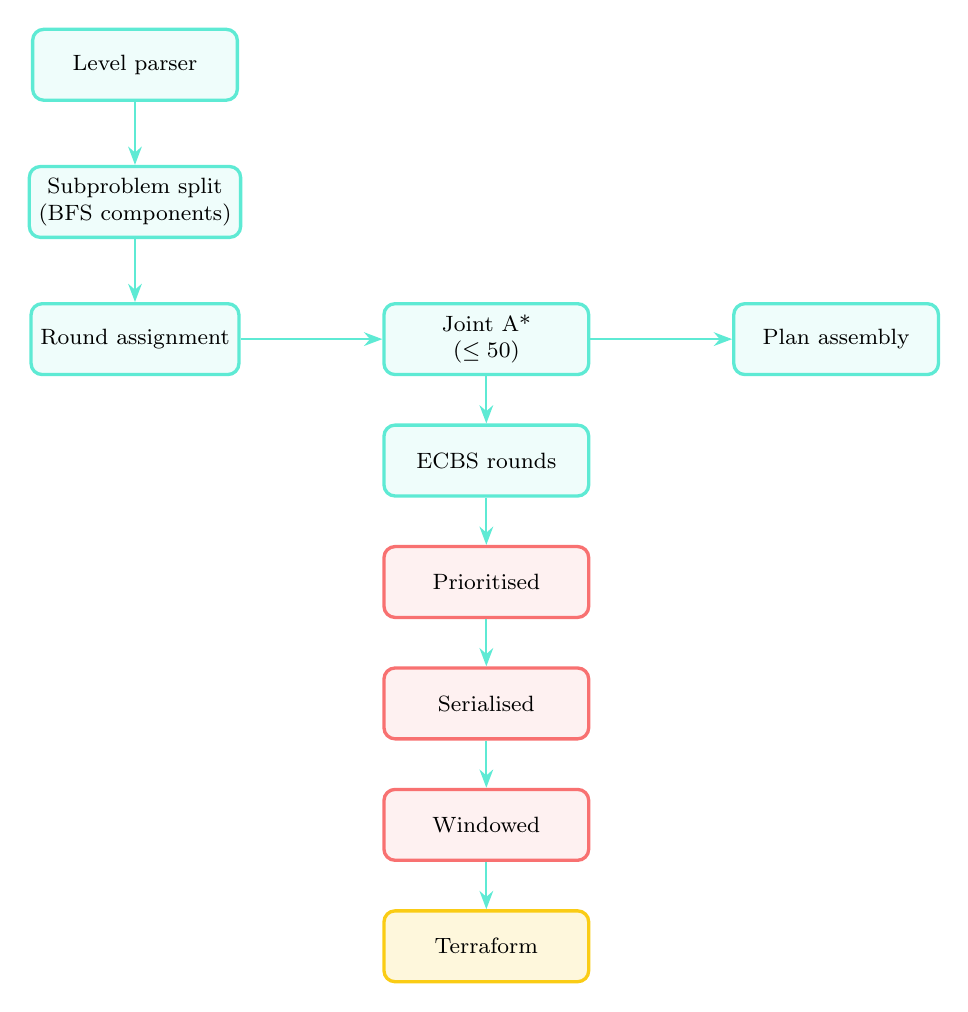
\begin{tikzpicture}[
        every node/.style={font=\footnotesize, align=center, rounded corners=4pt},
        box/.style={draw=accent, very thick, fill=accent!10, minimum width=2.6cm, minimum height=0.9cm},
        fallback/.style={draw=warn, very thick, fill=warn!10, minimum width=2.6cm, minimum height=0.9cm},
        last/.style={draw=accent2, very thick, fill=accent2!15, minimum width=2.6cm, minimum height=0.9cm},
        arr/.style={-{Stealth}, thick, accent},
      ]
      \node[box] (level) {Level parser};
      \node[box, below=8mm of level] (decomp) {Subproblem split\\(BFS components)};
      \node[box, below=8mm of decomp] (assign) {Round assignment};

      \node[box, right=18mm of assign] (joint) {Joint A*\\($\leq 50$)};
      \node[box, below=6mm of joint]    (ecbs)  {ECBS rounds};
      \node[fallback, below=6mm of ecbs] (prio) {Prioritised};
      \node[fallback, below=6mm of prio] (ser)  {Serialised};
      \node[fallback, below=6mm of ser]  (win)  {Windowed};
      \node[last, below=6mm of win]      (terra){Terraform};

      \node[box, right=18mm of joint] (assemble) {Plan assembly};

      \draw[arr] (level) -- (decomp);
      \draw[arr] (decomp) -- (assign);
      \draw[arr] (assign) -- (joint);
      \draw[arr] (joint)  -- (ecbs);
      \draw[arr] (ecbs)   -- (prio);
      \draw[arr] (prio)   -- (ser);
      \draw[arr] (ser)    -- (win);
      \draw[arr] (win)    -- (terra);
      \draw[arr] (joint)  -- (assemble);
    \end{tikzpicture}
  \end{center}

  \vspace{-0.2cm}
  \begin{center}
    \footnotesize\textcolor{muted}{Independence detection\citebadge{standley2010} · portfolio escalation\citebadge{leytonbrown2003}}
  \end{center}
\end{frame}

% --- 04 Subgoal decomposition ------------------------------------------
\begin{frame}{Subgoal decomposition}
  \begin{columns}[T, onlytextwidth]
    \column{0.62\textwidth}
      \screenshot{assets/images/decomposition_red_boundary.png}%
        {Level partitioned into independent sub-regions (red boundaries).}

    \column{0.36\textwidth}
      \vspace{1.2cm}
      \begin{itemize}
        \item BFS connected components on \emph{free} cells.
        \item Drop regions with no agent or goal.
        \item Each region solved independently, then re-assembled.
      \end{itemize}
      \vspace{0.6cm}
      \footnotesize\textcolor{muted}{Independence detection\citebadge{standley2010}}
  \end{columns}
\end{frame}

% --- 05 Joint-space A* --------------------------------------------------
\begin{frame}{Strategy 1 — Joint-space A*}
  \demovideo{assets/videos/joint_astar_demo.mp4}%
    {Weighted A* over joint actions; single OPEN list, $w = 2.5$.}

  \vspace{-0.1cm}
  \begin{center}
    \footnotesize\textcolor{muted}{Used when subproblem $\leq 50$ cells.\quad
      Weighted A*\citebadge{pohl1970} · coupled joint search\citebadge{standley2010}}
  \end{center}
\end{frame}

% --- 06 ECBS rounds -----------------------------------------------------
% Demo level: CphAirprt (10 agents, 33x44 airport-style layout, clean ECBS solve).
% Reserved for ECBS only — do not reuse on other slides.
\begin{frame}{Strategy 2 — Round-based ECBS}
  \vspace{-0.25cm}
  \begin{columns}[T, onlytextwidth]
    % --- LEFT: FOCAL diagram (small) ---
    \column{0.34\textwidth}
      \vspace{0.05cm}
      \begin{center}
        \begin{tikzpicture}[scale=0.85]
          \draw[draw=accent, very thick, fill=accent!8!slate]   (0,0)    circle (1.6);
          \draw[draw=accent2, very thick, fill=accent2!20!slate] (0,-0.25) circle (0.85);
          \node[font=\scriptsize\bfseries, accent]  at (0, 1.25) {OPEN};
          \node[font=\scriptsize\bfseries, accent2] at (0,-0.25) {FOCAL};
          \node[font=\tiny, muted] at (0,-0.85) {cost $\leq w\cdot$min};
          \node[font=\tiny, muted] at (0,-1.4)  {$w = 1.3$};
        \end{tikzpicture}
      \end{center}
      \vspace{-0.05cm}
      {\scriptsize\color{muted}\centering
        FOCAL picks the node with the \emph{fewest conflicts}.\par}

    % --- RIGHT: pseudocode + citations ---
    \column{0.64\textwidth}
      \vspace{0.05cm}
      \algbox{ECBS round}{%
        OPEN $\leftarrow$ \{root (no constraints)\}\\
        \textbf{while} OPEN $\neq \emptyset$ \textbf{do}\\
        \quad FOCAL $\leftarrow$ \{n $\in$ OPEN : n.cost $\leq w\cdot$min\}\\
        \quad n $\leftarrow$ pop FOCAL with fewest conflicts\\
        \quad c $\leftarrow$ first conflict in n.solution\\
        \quad \textbf{if} c is None \textbf{return} n.solution\\
        \quad \textbf{for} each agent in c: add constraint, replan, push}
      \vspace{0.1cm}

      {\scriptsize CBS\citebadge{sharon2015} · FOCAL\citebadge{barer2014} ·
       per-round re-assignment\citebadge{ma2017} ·
       route-blocking goal ordering\citebadge{felner2018}.\par}
  \end{columns}

  % --- BOTTOM: video placeholder ---
  \vspace{0.05cm}
  \demovideo[0.30\textheight]{assets/videos/06_ecbs_cphairprt_solve.mp4}%
    {\textbf{CphAirprt} — 10 agents · 33$\times$44 airport · cleanly solved by ECBS rounds.}
\end{frame}


% --- 07 ECBS fallbacks --------------------------------------------------
% Demo level: TwoPlayer (3 agents, narrow 3-cell passages → forces yielding).
% Reserved for fallback chain only.
\begin{frame}{When ECBS stalls — prioritised \,$\to$\, serialised}
  \vspace{-0.15cm}
  \begin{center}
    \begin{tikzpicture}[
      every node/.style={font=\footnotesize, align=center, rounded corners=5pt,
                         minimum width=2.9cm, minimum height=1.3cm, text=paper},
      arr/.style={-{Stealth}, thick, accent},
    ]
      \node[draw=accent, very thick, fill=accent!10!slate]
            (ecbs) {ECBS round\\{\tiny coupled, focal}};
      \node[draw=warn, very thick, fill=warn!10!slate, right=10mm of ecbs]
            (prio) {Prioritised\\{\tiny agent $i$ respects $<i$ reservations}};
      \node[draw=warn, very thick, fill=warn!15!slate, right=10mm of prio]
            (ser)  {Serialised\\{\tiny 1 mover, others static}};
      \draw[arr] (ecbs) -- node[above, font=\tiny\itshape, text=warn]
                              {budget exceeded} (prio);
      \draw[arr] (prio) -- node[above, font=\tiny\itshape, text=warn]
                              {still infeasible} (ser);
    \end{tikzpicture}
  \end{center}

  \vspace{0.1cm}
  \begin{columns}[T, onlytextwidth]
    % --- LEFT: pseudocode for the two fallbacks ---
    \column{0.46\textwidth}
      \algbox{prioritised}{%
        \textbf{for} agent $a_i$ in priority order:\\
        \quad respect reservations of $a_{<i}$\\
        \quad single-agent A*, write reservations}
      \\[6pt]
      \algbox{serialised}{%
        \textbf{for} agent $a_i$ in priority order:\\
        \quad freeze all other agents\\
        \quad single-agent A* on static map}
      \vspace{0.1cm}

      {\scriptsize
       Reservation tables\citebadge{erdmann1987}\citebadge{silver2005};
       serialised is always feasible if any single-agent plan exists\citebadge{erdmann1987}.\par}

    % --- RIGHT: short video showing sequential motion ---
    \column{0.50\textwidth}
      \demovideo[0.40\textheight]{assets/videos/07_fallback_twoplayer.mp4}%
        {\textbf{TwoPlayer} — 3 agents in 3-cell passages.\\
         Watch agents \emph{yield} for one another — the visual signature of
         prioritised / serialised motion.}
  \end{columns}
\end{frame}

% --- 08 Windowed joint A* ----------------------------------------------
\begin{frame}{Windowed joint A* — evict \& restore}
  \demovideo{assets/videos/windowed_demo.mp4}%
    {Rolling window around the delivery path; blocker moved aside, then restored if on its own goal.}

  \vspace{-0.1cm}
  \begin{center}
    \footnotesize\textcolor{muted}{Windowed Hierarchical Cooperative A*\citebadge{silver2005} ·
      Navigation Among Movable Obstacles\citebadge{stilman2005}}
  \end{center}
\end{frame}

% --- 09 Terraform -------------------------------------------------------
\begin{frame}{Multi-mover terraform — last resort}
  \demovideo{assets/videos/terraform_triwards.mp4}%
    {Scripted evict / vacate / deliver ops simulated step-by-step, executed by weighted joint A*.}

  \vspace{-0.1cm}
  \begin{center}
    \footnotesize\textcolor{muted}{Multi-Agent Terraforming\citebadge{vainshtein2022} ·
      internal mover uses weighted A*\citebadge{pohl1970}}
  \end{center}
\end{frame}

% --- 10 ClauDOom own level ---------------------------------------------
\begin{frame}{Our level: ClauDOom}
  \begin{columns}[T, onlytextwidth]
    \column{0.45\textwidth}
      \screenshot{assets/images/claudoom_level.png}{The ClauDOom level design.}
    \column{0.5\textwidth}
      \demovideo{assets/videos/claudoom_solve.mp4}{Our solver solving ClauDOom.}
  \end{columns}

  \vspace{0.2cm}
  \begin{itemize}
    \item TODO: design rationale (why these corridors / box density).
    \item TODO: which strategies our solver actually invokes here.
  \end{itemize}
\end{frame}

% --- 11 Experiments & tuning -------------------------------------------
\begin{frame}{Experiments \& tuning}
  \begin{center}
    \begin{tabular}{@{}l c l@{}}
      \toprule
      \textbf{Ablation} & \textbf{$\Delta$ solved} & \textbf{Why}\\
      \midrule
      remove Joint A* (only ECBS)        & TODO & small subproblems become slow \\
      cutoff $25 \to 50 \to 100$ cells   & TODO & sweet spot at $50$            \\
      $W_{\text{joint}} \in \{1.5, 2.5, 4\}$ & TODO & accuracy / speed trade-off \\
      remove Terraform                   & TODO & loses Nej, TriWards            \\
      remove FOCAL (plain CBS)           & TODO & blow-up on dense rooms         \\
      \bottomrule
    \end{tabular}
  \end{center}

  \vspace{0.4cm}
  \begin{center}
    \footnotesize\textcolor{muted}{Algorithm portfolio\citebadge{leytonbrown2003}}
  \end{center}
\end{frame}

% --- 12 Limitations -----------------------------------------------------
\begin{frame}{Limitations}
  \begin{itemize}
    \item TODO: levels we still fail on (e.g.\ \texttt{brAIn}, \texttt{sublevels}).
    \item TODO: terraform is scripted, not principled — brittle on dense rooms.
    \item TODO: ECBS focal width is fixed; no adaptive widening yet.
  \end{itemize}
\end{frame}

% --- 13 Future work -----------------------------------------------------
\begin{frame}{Future work}
  \begin{itemize}
    \item Principled TF-CBS (tMAPF refactor)\citebadge{vainshtein2022}.
    \item Adaptive focal widening when conflicts stagnate.
    \item Learned goal-ordering on top of \texttt{assignment.py}.
    \item TODO: more.
  \end{itemize}
\end{frame}

% --- 14 Competition results --------------------------------------------
\begin{frame}{Competition results}
  \begin{center}
    \screenshot{assets/images/competition_results.png}{Final standings — 64 teams.}
  \end{center}

  \vspace{-0.2cm}
  \begin{center}
    \resultcard{\faIcon{trophy}}{Overall}{73.78}{\#1 of 64}
    \quad
    \resultcard{\faIcon{medal}}{Actions}{34.21}{\#3 of 64}
    \quad
    \resultcard{\faIcon{stopwatch}}{Time}{39.58}{\#3 of 64}
  \end{center}

  \vspace{0.4cm}
  \begin{center}
    \Large\color{accent}\textbf{Thank you!}
  \end{center}
\end{frame}


% --- references appendix (not counted in the 12 min) ---
\appendix
\begin{frame}[allowframebreaks]{References}
  \tiny
  \printbibliography[heading=none]
\end{frame}

\end{document}
